\documentclass[11pt]{article}
\usepackage[paper=letterpaper, left=1in, right=1in, top=1in, bottom=1in]
           {geometry}
\usepackage[parfill]{parskip}
\usepackage{amsmath}
\usepackage{graphicx}
\usepackage{fancyvrb}
\usepackage{upquote}
\usepackage{xfrac}

\newcommand{\problem}[1]{\textbf{Problem #1 ---} }
\newcommand{\answer}{\textit{Answer: } }

\begin{document}
\thispagestyle{empty}

\begin{center}
{\large CS 310}\\
Assignment 131
\end{center}

\begin{flushright}
Karl Ramberg
\end{flushright}

\problem{1} Use the definitions to prove or disprove the statement
$n^4 - 2n^2 + 5 \in \Omega(n^3)$, and illustrate this graphically.

\answer The definition requires us to find $c$ and $n_0$ so that
\[
n^4 - 2n^2 + 5 \geq cn^3 \text{ when } n \geq n_0
\]

If this is true, then we can rearrange the inequality so that
\begin{align*}
\frac{n^4 - 2n^2 + 5}{n^3} \geq c \\
n - \frac{2}{n} + \frac{5}{n^3} \geq c
\end{align*}

We can then take the derivative of the left and find it's minimum by setting 
it equal to 0.

\begin{align*}
\frac{d}{dn}(n - \frac{2}{n} + \frac{5}{n^3}) = 0\\
1 + \frac{2}{n^2} - \frac{15}{n^4} = 0\\
n^4 + 2n^2 - 15 = 0\\
n = \sqrt{3}, -\sqrt{3}
\end{align*}

$\sqrt{3} \approx 1.731$ so we will choose $2$ for $n_0$, and $c \leq \frac{13}{8}$.
We will choose $1$ for $c$. 

This is graphically illustrated by the following plot that shows
$n^4 - 2n^2 + 5$ along with the standard function $n^3$ scaled by
the constant coefficient $c = 1$.

\begin{center}
  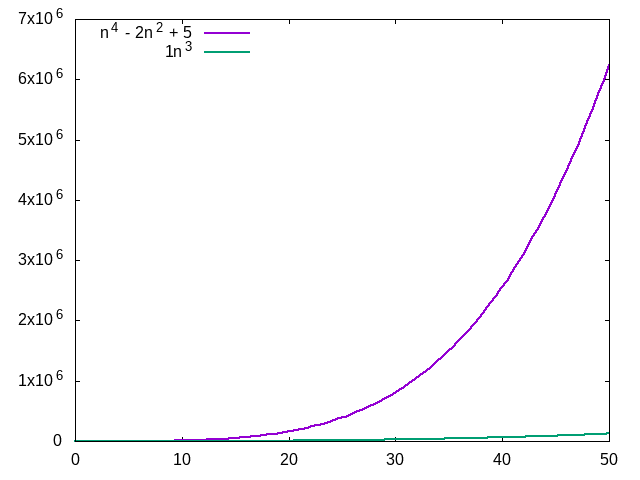
\includegraphics[width=0.7\textwidth]{problem1.png}
\end{center} 

\problem{2} Either prove the following assertion using the definitions
or disprove it with a specific counterexample:
\[
\text{if } T(n) \in O(f(n)) \text{ then } f(n) \in \Omega(T(n))
\]

\answer If we assume $T(n) \in O(f(n))$ them we can assume there is a $c > 0$ 
and $n > n_0$ such that $T(n) \leq c*f(n)$.

If we rearrange this inequality, we find that $f(n) \geq \frac{1}{c} * T(n)$.

Since $c > 0$ we can assume $\frac{1}{c} > 0$ and can rename it to $c_2$.

So we write $f(n) \geq c_2 * T(n)$. This satisfies the definition of 
$\Omega(n)$, which means $f(n) \in \Omega(T(n))$.


\problem{3} For the following algorithm, explain what it computes,
state what the input size for analysis is, state what basic operations
should be counted for analyzing it, state exactly how many operations
are executed as a function of the input size, and state the efficiency
class to which it belongs.

\begin{Verbatim}[numbers=left,xleftmargin=5mm]
void foo(vector<unsigned>& array)
{
  for (size_t pass_indx = array.size() - 1; pass_indx > 0; pass_indx--)
  {
    for (size_t compare_indx = 0; compare_indx < pass_indx; compare_indx++)
    {
      if (array.at(compare_indx) > array.at(compare_indx + 1))
      {
        swap(array.at(compare_indx), array.at(compare_indx + 1));
      }
    }
  }
}
\end{Verbatim}

\answer This algorithm is a simple bubble sort. It takes an array an performs 
swaps when it sees elements out of order.
The input size, $n$, for this algorithm will simply be the size of the vector.

The outer \texttt{for} loop will have $2(n-1)$ instructions.

The inner \texttt{for} loop will run $2(n-1)$ instructions the first time and 
$2(n-1)$ the next, and so on for n times. As a formal series this is
$\sum_{i=1}^{n-1} (2(n-i))$ instructions. Since $\sum_{i=1}^{n-1} (2(n-i))
= \frac{n(n-1)}{2} = \frac{1}{2}(n^2-n)$, this will be our highest order term at $n^2$.

The inner \texttt{if} statement will run an extra 2 or 4 instructions every
time the inner \texttt{for} loop runs. This doesn't effect the complexity.

The best case (already sorted) formula is
\[
2n + \sum_{i=1}^{n-1} (2(n-i) + 2)
\]
The worst case (reverse order) formula is
\[
2n + \sum_{i=1}^{n-1} (2(n-i) + 4)
\]

The efficiency of this algorithm is $T(n) \in \Theta(n^2)$.
Since this algorithm will run all the way through every time both the best and
worst case have the same complexity.


\problem{4} Write a C++ program that implements the algorithm
in problem 3, counts the number of basic operations, and outputs the
input size and the count of basic operations to the cerr stream. Run
this program many times with many different inputs and capture the
results.

\answer See the submitted file \texttt{rambergk131.cpp}.


\problem{5} Using the output of the program in Problem 4, create a
plot of input size vs.\ basic operations, along with one or more
standard functions properly scaled, to illustrate your analysis in
Problem 3.

\answer When the program is run with the command

\begin{Verbatim}
for n in `seq 1 10 1000`;
do 
  ./rambergk131 $n;
done 1> /dev/null 2> results.dat
\end{Verbatim}

and the resulting data file is plotted with gnuplot, the following is
produced. Also plotted on the same axes is the standard
function $n^2$ scaled by $1.5$ and $2.5$ which illustrates that
\[
T(n) \in \Theta(n^2)\\
\]

\begin{center}
  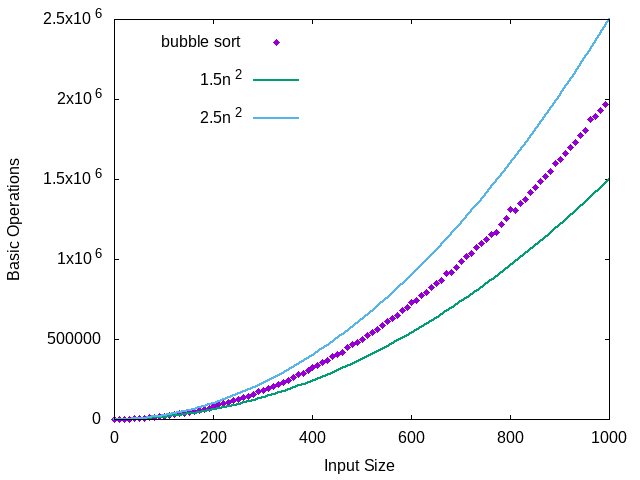
\includegraphics[width=0.7\textwidth]{problem5.png}
\end{center} 

\end{document}

%%  LocalWords:  cn Yada yada indx cerr cpp dat
